\chapter{PILOT USER STUDY} \label{sec:userstudy}
Aside from creating an online architectural interface for simulations, I also made preparations for a pilot user study aimed at answering a few evaluation questions about the usability of our online interface.  I hypothesize that if OASIS is publicized to users online, then anonymous online users will construct models in our sketching interface and create daylight renderings for analysis.  Additionally, this pilot user study will serve as a test for OASIS.  In theory there should be no issues when multiple users are logged into OASIS; However, OASIS has yet to be used by multiple users simultaneously.  To summarize, I anticipate  that this pilot user study will provide us valuable feedback to improve OASIS.  \\

\section{Previous User Studies}
% Point I'm trying to get across is that OASIS will make collecting models easy. Just make the point.	
The physical sketch interpretation algorithm has gone through three previous user studies.  The physical sketch interpretation algorithm has gone through three previous user studies.  While these previous studies gathered over 300 physical sketches, they did so from a medium sized pool of users.  This pool of users varied from 13 to 30 participants across all previous user studies.  It is also important to note that these studies each took, on average, 2 months to complete data collection and were comprised of mostly students at Rensselaer Polytechnic Institute.  The cost of effort to collect a model is relativity high compared to OASIS.  Overall I speculate that the number of models produced on OASIS will be quantitatively larger  and from a broader range of users than previous user studies.  \\

\section{Availability Of OASIS}
% OASIS can be used by anyone who is interested
In order to provide an architectural sketching interface for both novices and experts,  we must support as many platforms as possible. While experts my go to great lengths to install a piece of software, novices might not expend as much effort or have the technical skills required to install software.  As a result of being a web application OASIS is platform independent, has no installation process, and can globally apply updates to all clients.  Additionally, having a web application lends itself naturally to using a client-server architecture.  In OASIS I leverage the server to both service our web page and run computationally expensive processes on behalf of clients.  Namely, these computationally expensive processes are the physical sketch interpretation algorithm and the daylight rendering engine.  Both of these processes are computed on a specialized lab machine rather then locally on users' machines.  My hope is that leveraging the server to run computationally expensive components in OASIS will prevent potential participants from opting out of our pilot user study due to hardware limitations and will provide a homogeneous user experience across all platforms.  \\


\section{User Feedback  Collection In OASIS}
% This section should be strictly about what we collect, not how we collect it.
In OASIS I collect two types of data from users. Both active and passive data are collected from users while they use our tool. Active data refers to the feedback, models, and comments users actively provide. The relationship between users, models, renovations, and renderings can be seen in Figure-\ref{fig:rel}. Passive data refers to data not actively provided by users, such as the length of time a user spends on a page, the average wait time before rendering request are handled, and other information about users usage of our application. We collect both types of data to get a clearer idea of how users perceive OASIS and how users interact with our tool. Active feedback data collected is associated with either a specific user, model, renovation, or rendering in OASIS. This includes questions pertaining to users' past experience and education in fields such as architecture and the visual arts. Additionally, we are interested in users experience with other 3D modeling or simulation tools for architecture. We also ask users questions pertaining to their sketches. For example, we ask users to categorize their sketches; daylighting practices vary for bedrooms, offices, classrooms, and more. Understanding what kind of space a user is sketching is important for future analysis.	Aside from asking users to categorize their sketches, we also ask users to elaborate on how confident they are in their accuracy of their sketches.  While, I might not be interested in users' confidence in recreating sketches in this pilot user study, future studies can compare users' created sketches to real blue prints to gain insight into how users perceive and sketch architectural spaces from memory.  \\

We are also interested in collecting feedback on model renovations. Particularly, we are interested in if the 3D models generated by the physical sketch interpretation algorithm matches users' original intentions. As stated previously, the physical sketch interpretation algorithm usually matches users' intentions, however there are cases where  3D models generated is not representative of users' original intentions. Users can make modifications to models, defined as renovations, for a variety of reasons. They could be trying to alter the distribution of daylight in their architectural space or trying to better communicate their intentions to the physical sketch interpretation algorithm. Lastly, we ask users questions about renderings they created. Some questions generally ask about the effectiveness of OASIS as a daylight analysis tool; Other questions are more specific such as if a user understands the results of a particular rendering. All questions presented to users can be viewed in Chapter-\ref{sec:appendix}.  \\

				
As mentioned before we also collect passive data.  Specifically, we collect how long users spend on each page of our interface and how long users wait for both  sketch interpretations and daylight renderings.  \\

\begin{figure}[h]
\centering
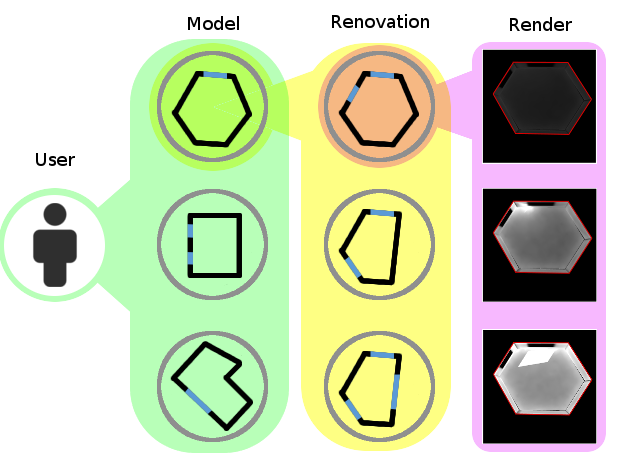
\includegraphics[width=0.8\textwidth]{relationship}
\caption[The relationship between users, models, renovations, and renderings.]{The relationship between users, models, renovations, and renderings. Users are associated with a set of models, models are associated with a set of renovations, and renovations are associated with a set of renderings.}
\label{fig:rel}	
\end{figure}


\section{Data Collection}
In order to collect feedback on OASIS we have to first host the application online, and then bring potential users' attention to the application. As an online study, we must invite users to participate in order to collect feedback.  Personally inviting individuals to use our tool might be cumbersome and slow going, so we hope inviting users in large groups by advertising in social media networks and on online bulletin boards will result in increased user participation. One advantage of using online bulletin boards is that they are organized by users' interest.  We use this organization to target users who might have an interest in daylighting or architecture. For this study we focused on advertising on  Reddit\footnote{https://www.reddit.com/[Accessed: Apr 8 2016]}. Reddit is a popular online bulletin board where users organize themselves by interest into smaller bulletin boards known as subreddits. In these subreddits users can share content such as links, images, and text that is relevant to the subreddits's interest. Table-\ref{fig:reddit} list a few relevant subreddits and their respective user sizes that we plan to advertise OASIS to.  \\
	
\begin{table}[ht!]
\centering
\caption{Subreddits and their respective subscribers sizes.}
\label{fig:reddit}
\begin{tabular}{ | l | l | }
\hline
Subreddit               & Subscribers  \\ \hline
InteriorDesign 			& 78,750        \\ \hline
RPI 			        & 3,939         \\ \hline
Floorplan    			& 1,175         \\ \hline
UserExperienceDesign    & 1,128         \\ \hline
GreenArchitecture 		& 607          \\ \hline
YoungArchitects 		& 236          \\ \hline
\end{tabular}
\end{table}

Additionally, in this pilot study we target users who are likely to create models of Rensselaer Polytechnic Institute dormitories. If a user communicates that they are sketching an RPI dormitory by answering feedback questions, we ask the user to elaborate on which RPI dormitory they are sketching. We are collecting this data for future studies where we can analyze users' sketches of RPI dormitories against blue prints of those dormitories. Doing so would give us insight into how accurately users can sketch their dormitories. To begin, we plan on advertising OASIS on a subreddit unofficially affiliated with RPI. Moreover, we plan on also advertising our tool on campus. As done in previous studies we wish to leverage the Rensselaer Polytechnic Institute School of Architecture in order to collect feedback from users with formal education in architecture. Students with formal education in architecture are likely to have experience with architectural design software and daylighting. Their feedback, as non-novices, I believe will be useful because their previous experience with related software can help us improve OASIS.  \\

\section{Chapter Summary}

In addition to the creation of OASIS, I also conducted a pilot user study.  I hypothesize that if OASIS is publicized to users online, then anonymous online users will construct models in our sketching interface and create daylight renderings for analysis.  Also, I speculate that the number of models anonymous online users will construct on OASIS will be quantitatively larger and from a broader range of users than previous user studies conducted on the Virtual Heliodon.  Collecting both active and passive feedback from users will help us better understand where improvements to OASIS can be made and how users currently experience OASIS.  Lastly, in order to collect as much feedback as possible we plan on advertising OASIS on social media outlets, online bulletin boards, and on campus.  To summarize, I anticipate  that this pilot user study will provide us valuable feedback to improve OASIS.  \\


